% @Author: Taha Bouhsine


%%%%%%%%%%%%%%%%%%%%%%%%%%%%
% CHAPTER                  %
%%%%%%%%%%%%%%%%%%%%%%%%%%%%
\setcounter{mtc}{11}

\chapter{Realization, GUI And Tests}%
\label{chap:chapter_four}
\minitoc

\section{Hardware environments}


\section{Development Environments}
\subsection{Design And Planing}

\paragraph{PlantUml}
PlantUML is an open-source tool allowing users to create UML diagrams from plain text language. The language of PlantUML is an example of a Domain-specific language. It uses Graphviz software to lay out its diagrams. It has been used to allow blind students to work with UML. PlantUML also helps blind software engineers to design and read UML diagrams.


\paragraph{Gantt chart}
A Gantt chart is a horizontal bar chart that visually represents a project plan over time. Modern Gantt charts typically show us the status of—as well as who’s responsible for—each task in the project.

In other words, a Gantt chart is a super-simple way to keep us out of a project pinch!

What are the key parts of a Gantt chart?
A Gantt chart is made up of several different elements:
\begin{enumerate}
      \item
            Tasklist: Runs vertically down the left of the Gantt chart to describe project work and may be organized into groups and subgroups
      \item
            Timeline: Runs horizontally across the top of the Gantt chart and shows months, weeks, days, and years
      \item
            Dateline: A vertical line that highlights the current date on the Gantt chart
      \item
            Bars: Horizontal markers on the right side of the Gantt chart that represent tasks and show progress, duration, and start and end dates
      \item
            Milestones: Yellow diamonds that call out major events, dates, decisions, and deliverables
      \item
            Dependencies: Light gray lines that connect tasks that need to happen in a certain order
      \item
            Progress: Shows how far along work is and may be indicated by \% Complete and/or bar shading
      \item
            Resource assigned: Indicates the person or team responsible for completing a task
\end{enumerate}


\subsection{Design}
\paragraph{Adobe Photoshop}
Adobe Photoshop is a software application for image editing and photo retouching for use on Windows or macOS computers. Photoshop offers users the ability to create, enhance, or otherwise edit images, artwork, and illustrations. Changing backgrounds, simulating a real-life painting, or creating an alternative view of the universe are all possible with Adobe Photoshop. It is the most widely used software tool for photo editing, image manipulation, and retouching for numerous image and video file formats. The tools within Photoshop make it possible to edit both individual images as well as large batches of photos.
We used it to prototype and create our platform logo.
\paragraph{Adobe XD}
Adobe XD is a vector-based user experience design tool for web apps and mobile apps, developed and published by Adobe Inc. It is available for macOS and Windows, although there are versions for iOS and Android to help preview the result of work directly on mobile devices. XD.












\subsection{Development}
\subsubsection{Version Control}
When building software it’s always important to track your changes. This is especially critical when collaborating on projects where multiple people will be updating the same code. Software that can keep track of all
these changes is called Version Control. The Version Control software we used is called Git. Because we built
the platform for a client we decided to get a private repository at Github.com.

\paragraph{Git}
% Git is a version control system for tracking changes in computer files and coordinating work on those files among multiple people. It is primarily used for source code management in software development, but it can be used to keep track of changes in any set of files. As a distributed revision control system it is aimed at speed, data integrity, and support for distributed, non-linear workflows.
Git is a distributed revision control and source code management system that
allows several people to work on the same codebase at the same time on different
computers and networks. These can be pushed together, with all changes stored and
recorded. It’s also possible to roll back to an earlier state if necessary.
\paragraph{Github}
At a high level, GitHub is a website and cloud-based service that helps developers store and manage their code, as well as track and control changes to their code. To understand exactly what GitHub is, we need to know two connected principles:
\begin{enumerate}
      \item Version control
      \item Git
\end{enumerate}

\paragraph{Github Desktop}
GitHub Desktop is a fast and easy way to contribute to projects from Windows and OS X, whether we are seasoned users or new users, GitHub Desktop is designed to simplify all processes and workflow in our GitHub. GitHub Desktop is an open-source Electron-based GitHub app. It is written in TypeScript and uses React.


\subsubsection{Dependency Managers}
A large software project often makes use of many third-party packages and libraries. In turn, these packages
often rely on several other packages and so on. To keep track of all these dependencies, software developers
use package managers. Below we introduce the ones we have used.
\paragraph{NPM}
\paragraph{Angular CLI}

\subsubsection{IDEs}

\paragraph{Visual Studio Code}
DescriptionVisual Studio Code is a source code editor developed by Microsoft for Windows, Linux and macOS. It includes support for debugging, embedded Git control and GitHub, syntax highlighting, intelligent code completion, snippets, and code refactoring.


\paragraph{MongoDB Compass Community}
MongoDB Compass is the defacto GUI tool for MongoDB much like MySQL Workbench is MySQL’s associated tool. It allows us to visually explore our data, run ad hoc queries, interact with our data with full CRUD functionality, as well as view and optimize our queries’ performance.


\paragraph{Postman}
Postman is an interactive and automatic tool for verifying the APIs of our project. Postman is a Google Chrome app for interacting with HTTP APIs. It presents us with a friendly GUI for constructing requests and reading responses. It works on the backend, and makes sure that each API is working as intended.

In Postman, we create a request, and Postman looks at the response to make sure it has the element we want in it. As it is an automation tool, it drastically improves the testing time and quality of the project. It helps in the early detection of bugs that might sprout at later stages and cause more damage to the system.

Postman is the way to streamline the process of API testing. All APIs that we create and deploy first rigorously go through Postman so that any major or show stopper bugs are identified on time and fewer bugs leak through to later stages.




\subsubsection{Report And Presentation}
\paragraph{Boost Note}
Boostnote is an Open source note-taking app for programmers.
Boostnote is a niche tool because designed for programmers, but we are passionate for it.
It focuses on writing Markdown notes and code snippets quickly, and get organized in a better way.

\paragraph{Latex}
\latex{} is a tool used to create professional-looking documents. It is based on the WYSIWYM (what we see is what we mean) idea, meaning we only have to focus on the contents of our document and the computer will take care of the formatting. Instead of spacing out text on a page to control formatting, as with Microsoft Word or LibreOffice Writer, users can enter plain text and let LATEX take care of the rest.
\paragraph{MiKTex}
MiKTeX provides the tools necessary to prepare documents using the TeX/LaTeX markup language, as well as a simple tex editor: TeXworks.

\paragraph{Tex Live}
TeX Live is intended to be a straightforward way to get up and running with the TeX document production system. It provides a comprehensive TeX system with binaries for most flavors of Unix, including GNU/Linux, macOS, and also Windows. It includes all the major TeX-related programs, macro packages, and fonts that are free software, including support for many languages around the world. Many operating systems provide it via their distributions.



\paragraph{Markdown}
Markdown is a lightweight markup language with plain-text-formatting syntax. Its design allows it to be converted to many output formats, but the original tool by the same name only supports HTML. Markdown is often used to format readme files, for writing messages in online discussion forums, and to create rich text using a plain text editor.
\paragraph{Marp}
Marp is the ecosystem to write our presentation with plain Markdown.


% section
% section
% section
\section{Frameworks}
\subsection*{MEAN stack}

\begin{figure}[!ht]
      \center
      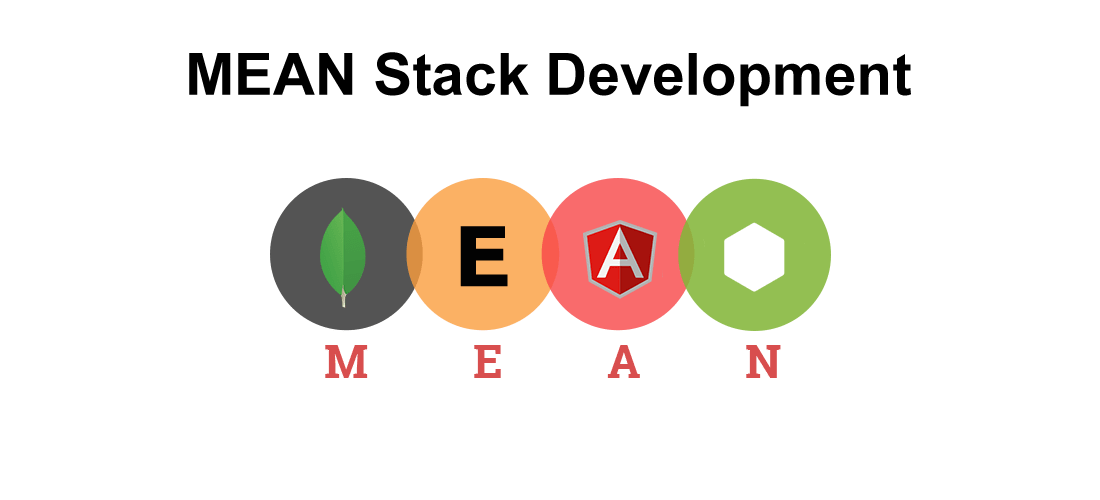
\includegraphics[scale=0.30]{assets/meanstack.png}
\end{figure}

While the name sounds like “mean”, it stands for the software pieces that are used to create a particular development stack: MongoDB, ExpressJS, Angular, and NodeJS. One of the biggest advantages of using this particular development stack is the ability to allow developers to use one consistent data model across the stack, using \ac{JSON} and BSON (for MongoDB). This allows for quick transitions between the various pieces of the stack, especially when a single programmer has to handle more than one portion of the stack.

\begin{figure}[!ht]
      \center
      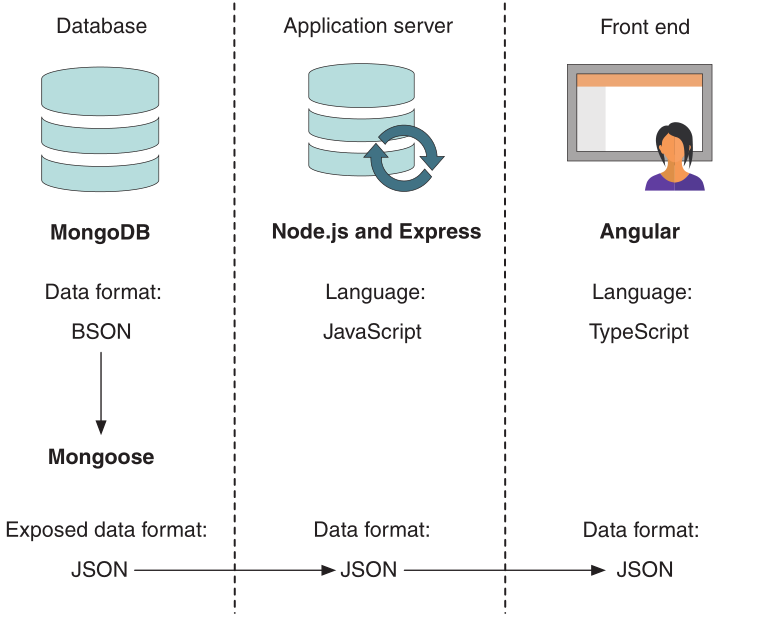
\includegraphics[scale=0.60]{assets/mean.png}
      \caption{Mean Stack}
      \label{fig:mean}
\end{figure}
\subsection{Front-End}
\subsubsection{Single Page Application}
Single-page application \ac{SPA} is an app that works inside a browser and does not require page reloading during use. You are using this type of applications every day. These are, for instance: Gmail, Google Maps, Facebook or GitHub.
SPAs are all about serving an outstanding UX by trying to imitate a “natural” environment in the browser — no page reloads, no extra wait time. It is just one web page that you visit which then loads all other content using JavaScript — which they heavily depend on.
SPA requests the markup and data independently and renders pages straight in the browser. We can do this thanks to the advanced JavaScript frameworks like AngularJS, Ember.js, Meteor.js, Knockout.js .
Single-page sites help keep the user in one, comfortable web space where content is presented to the user in a simple, easy and workable fashion.
\paragraph{Pros}
\begin{enumerate}
      \item 
      SPA is fast, as most resources (HTML+CSS+Scripts) are only loaded once throughout the lifespan of application. Only data is transmitted back and forth.
      \item 
      The development is simplified and streamlined. There is no need to write code to render pages on the server. It is much easier to get started because you can usually kick off development from a file file://URI, without using any server at all.
      \item 
      SPAs are easy to debug with Chrome, as you can monitor network operations, investigate page elements and data associated with it.
      \item 
      It’s easier to make a mobile application because the developer can reuse the same backend code for web application and native mobile application.
      \item 
      SPA can cache any local storage effectively. An application sends only one request, store all data, then it can use this data and works even offline.
\end{enumerate}
\subsubsection{Angular 9}
Angular is an app-design framework and development platform for creating efficient and sophisticated single-page apps in html, css, and Typescript which is a superset of JavaScript. Angular provides built-in features for animation, http service, and materials which in turn have features such as auto-complete, navigation, toolbar, menus, etc. The code is written in Typescript, which compiles to JavaScript and displays the same in the browser.

\subsection{Back-End}
\paragraph{Node Js}
Node.js is open-source, and a cross-platform runtime environment for developing server-side and networking applications. Node.js applications are written in JavaScript, and can be run within the Node.js runtime on OS X, Microsoft Windows, and Linux.
Node.js also provides a rich library of various JavaScript modules which simplifies the development of web applications using Node.js to a great extent.

The following are some of the important features that make Node.js the first choice of software architects.
\begin{enumerate}
      \item
            Asynchronous and Event-Driven: All APIs of Node.js library are asynchronous, that is, non-blocking. It essentially means a Node.js based server never waits for an API to return data. The server moves to the next API after calling it and a notification mechanism of Events of Node.js helps the server to get a response from the previous API call.
      \item
            Very Fast: Being built on Google Chrome's V8 JavaScript Engine, Node.js library is very fast in code execution.
      \item
            Single-Threaded but Highly Scalable: Node.js uses a single-threaded model with event looping. The event mechanism helps the server to respond in a non-blocking way and makes the server highly scalable as opposed to traditional servers which create limited threads to handle requests. Node.js uses a single-threaded program and the same program can provide service to a much larger number of requests than traditional servers like Apache HTTP Server.
      \item
            No Buffering: Node.js applications never buffer any data. These applications simply output the data in chunks.
      \item
            License: Node.js is released under the MIT license
\end{enumerate}



\paragraph{Express Js}
ExpressJS is a web application framework that provides us with a simple API to build websites, web apps, and back ends. With ExpressJS, we need not worry about low-level protocols, processes, etc.
Express provides a minimal interface to build our applications. It provides us the tools that are required to build our app. It is flexible as there are numerous modules available on npm, which can be directly plugged into Express.
Express was developed by TJ Holowaychuk and is maintained by the Node.js Foundation and numerous open source contributors.



\paragraph{MongoDB}
MongoDB is a cross-platform, document-oriented database that provides, high performance, high availability, and easy scalability. MongoDB works on the concept of collection and document.
\begin{enumerate}
      \item
            Database\\
            The database is a physical container for collections. Each database gets its own set of files on the file system. A single MongoDB server typically has multiple databases.
      \item
            Collection\\
            A collection is a group of MongoDB documents. It is the equivalent of an RDBMS table. A collection exists within a single database. Collections do not enforce a schema. Documents within a collection can have different fields. Typically, all documents in a collection are of similar or related purposes.
      \item
            Document\\
            A document is a set of key-value pairs. Documents have a dynamic schema. Dynamic schema means that documents in the same collection do not need to have the same set of fields or structures, and common fields in a collection's documents may hold different types of data.
\end{enumerate}


\paragraph{Mongoose}
Mongoose is an Object Data Modeling (ODM) library for MongoDB and Node.js. It manages relationships between data, provides schema validation, and is used to translate between objects in code and the representation of those objects in MongoDB.





% section
% section
% section





\section{Programming Languages}

\subsection{Conception}
\paragraph{Unified Modeling Language}

\subsection{General}
\paragraph{JavaScript Object Notation}
\ac{JSON} is a lightweight data-interchange format. It is easy for humans to read and write. It is easy for machines to parse and generate. It is based on a subset of the JavaScript Programming Language Standard ECMA-262 3rd Edition - December 1999. \ac{JSON} is a text format that is completely language independent but uses conventions that are familiar to programmers of the C-family of languages, including C, C++, C\#, Java, JavaScript, Perl, Python, and many others. These properties make \ac{JSON} an ideal data-interchange language.

\subsection{Front-End}
\paragraph{Typescript}
TypeScript is an open-source programming language developed and maintained by Microsoft. It is a strict syntactical superset of JavaScript and adds optional static typing to the language. TypeScript is designed for the development of large applications and transcompiles to JavaScript. As TypeScript is a superset of JavaScript, existing JavaScript programs are also valid TypeScript programs.

TypeScript may be used to develop JavaScript applications for both client-side and server-side execution (as with Node.js or Deno). There are multiple options available for transcompilation. Either the default TypeScript Checker can be used, or the Babel compiler can be invoked to convert TypeScript to JavaScript.

TypeScript supports definition files that can contain type information of existing JavaScript libraries, much like C++ header files can describe the structure of existing object files. This enables other programs to use the values defined in the files as if they were statically typed TypeScript entities. There are third-party header files for popular libraries such as jQuery, MongoDB, and D3.js. TypeScript headers for the Node.js basic modules are also available, allowing the development of Node.js programs within TypeScript.

The TypeScript compiler is itself written in TypeScript and compiled to JavaScript. It is licensed under the Apache License 2.0. TypeScript is included as a first-class programming language in Microsoft Visual Studio 2013 Update 2 and later, besides C\# and other Microsoft languages. An official extension allows Visual Studio 2012 to support TypeScript as well. Anders Hejlsberg, the lead architect of C\# and creator of Delphi and Turbo Pascal, has worked on the development of TypeScript.

\paragraph{HTML}
Hypertext Markup Language \ac{HTML} is the standard markup language for documents designed to be displayed in a web browser. It can be assisted by technologies such as Cascading Style Sheets (CSS) and scripting languages such as JavaScript.

Web browsers receive HTML documents from a web server or local storage and render the documents into multimedia web pages. HTML describes the structure of a web page semantically and originally included cues for the appearance of the document.



\paragraph{CSS}
Cascading Style Sheets \ac{CSS} is a style sheet language used for describing the presentation of a document written in a markup language like HTML. CSS is a cornerstone technology of the World Wide Web, alongside HTML and JavaScript.

\ac{CSS} is designed to enable the separation of presentation and content, including layout, colors, and fonts. This separation can improve content accessibility, provide more flexibility and control in the specification of presentation characteristics, enable multiple web pages to share formatting by specifying the relevant CSS in a separate .css file, and reduce complexity and repetition in the structural content.


\subsection{Back-End}
\paragraph{Javascript}
JavaScript often abbreviated as JS, is a programming language that conforms to the ECMAScript specification. JavaScript is high-level, often just-in-time compiled, and multi-paradigm. It has curly-bracket syntax, dynamic typing, prototype-based object-orientation, and first-class functions.
\paragraph{ES6}
Script. The developers use ECMAScript mostly for client-side scripting of the World Wide Web \ac{WWW}.

The sixth edition of the ECMAScript standard is ECMAScript6 or ES6 and later renamed as ECMAScript 2015. It is a major enhancement to the JavaScript language, which allows us to write programs for complex applications. It adds many features intended to make large-scale software development easier. The most common ES6 web-browsers are Chrome and Firefox. A transpiler converts the ES6 based code into ES5 which is supported many browsers. TypeScript is a transpiler. Grunt, Gulp, and Babel are some other transpilers to compile the modules. Therefore, TypeScript supports ES6.


% section
% section
% section

\section{Platform security}
\subsection{Physical level}
\subsection{Logical level}
\paragraph{JWT}
\paragraph{HTTP}

% section
% section
% section

\section{Interfaces}
% section
% section
% section

\section{tests}

% section
% section
% section
% section

\section{Deployment}

